% In order to have an accurate upper bound of the  adaptivity of a program $c$,
% we design a
This part gives the architecture overview for this 
% The 
new program analysis framework, named {\THESYSTEM}.
% It 
Specifically, it can be divided as the following steps:
1) statically analyzes the program's data dependency relation;
2) statically analyzes the program's dependency quantity properties;
3) constructs a weighted dependency graph based on $c$ using the two analysis results above; 
4) then finds a path in this graph, which is used to estimate an upper bound on the adaptivity of $c$.
\begin{figure}
  \centering    
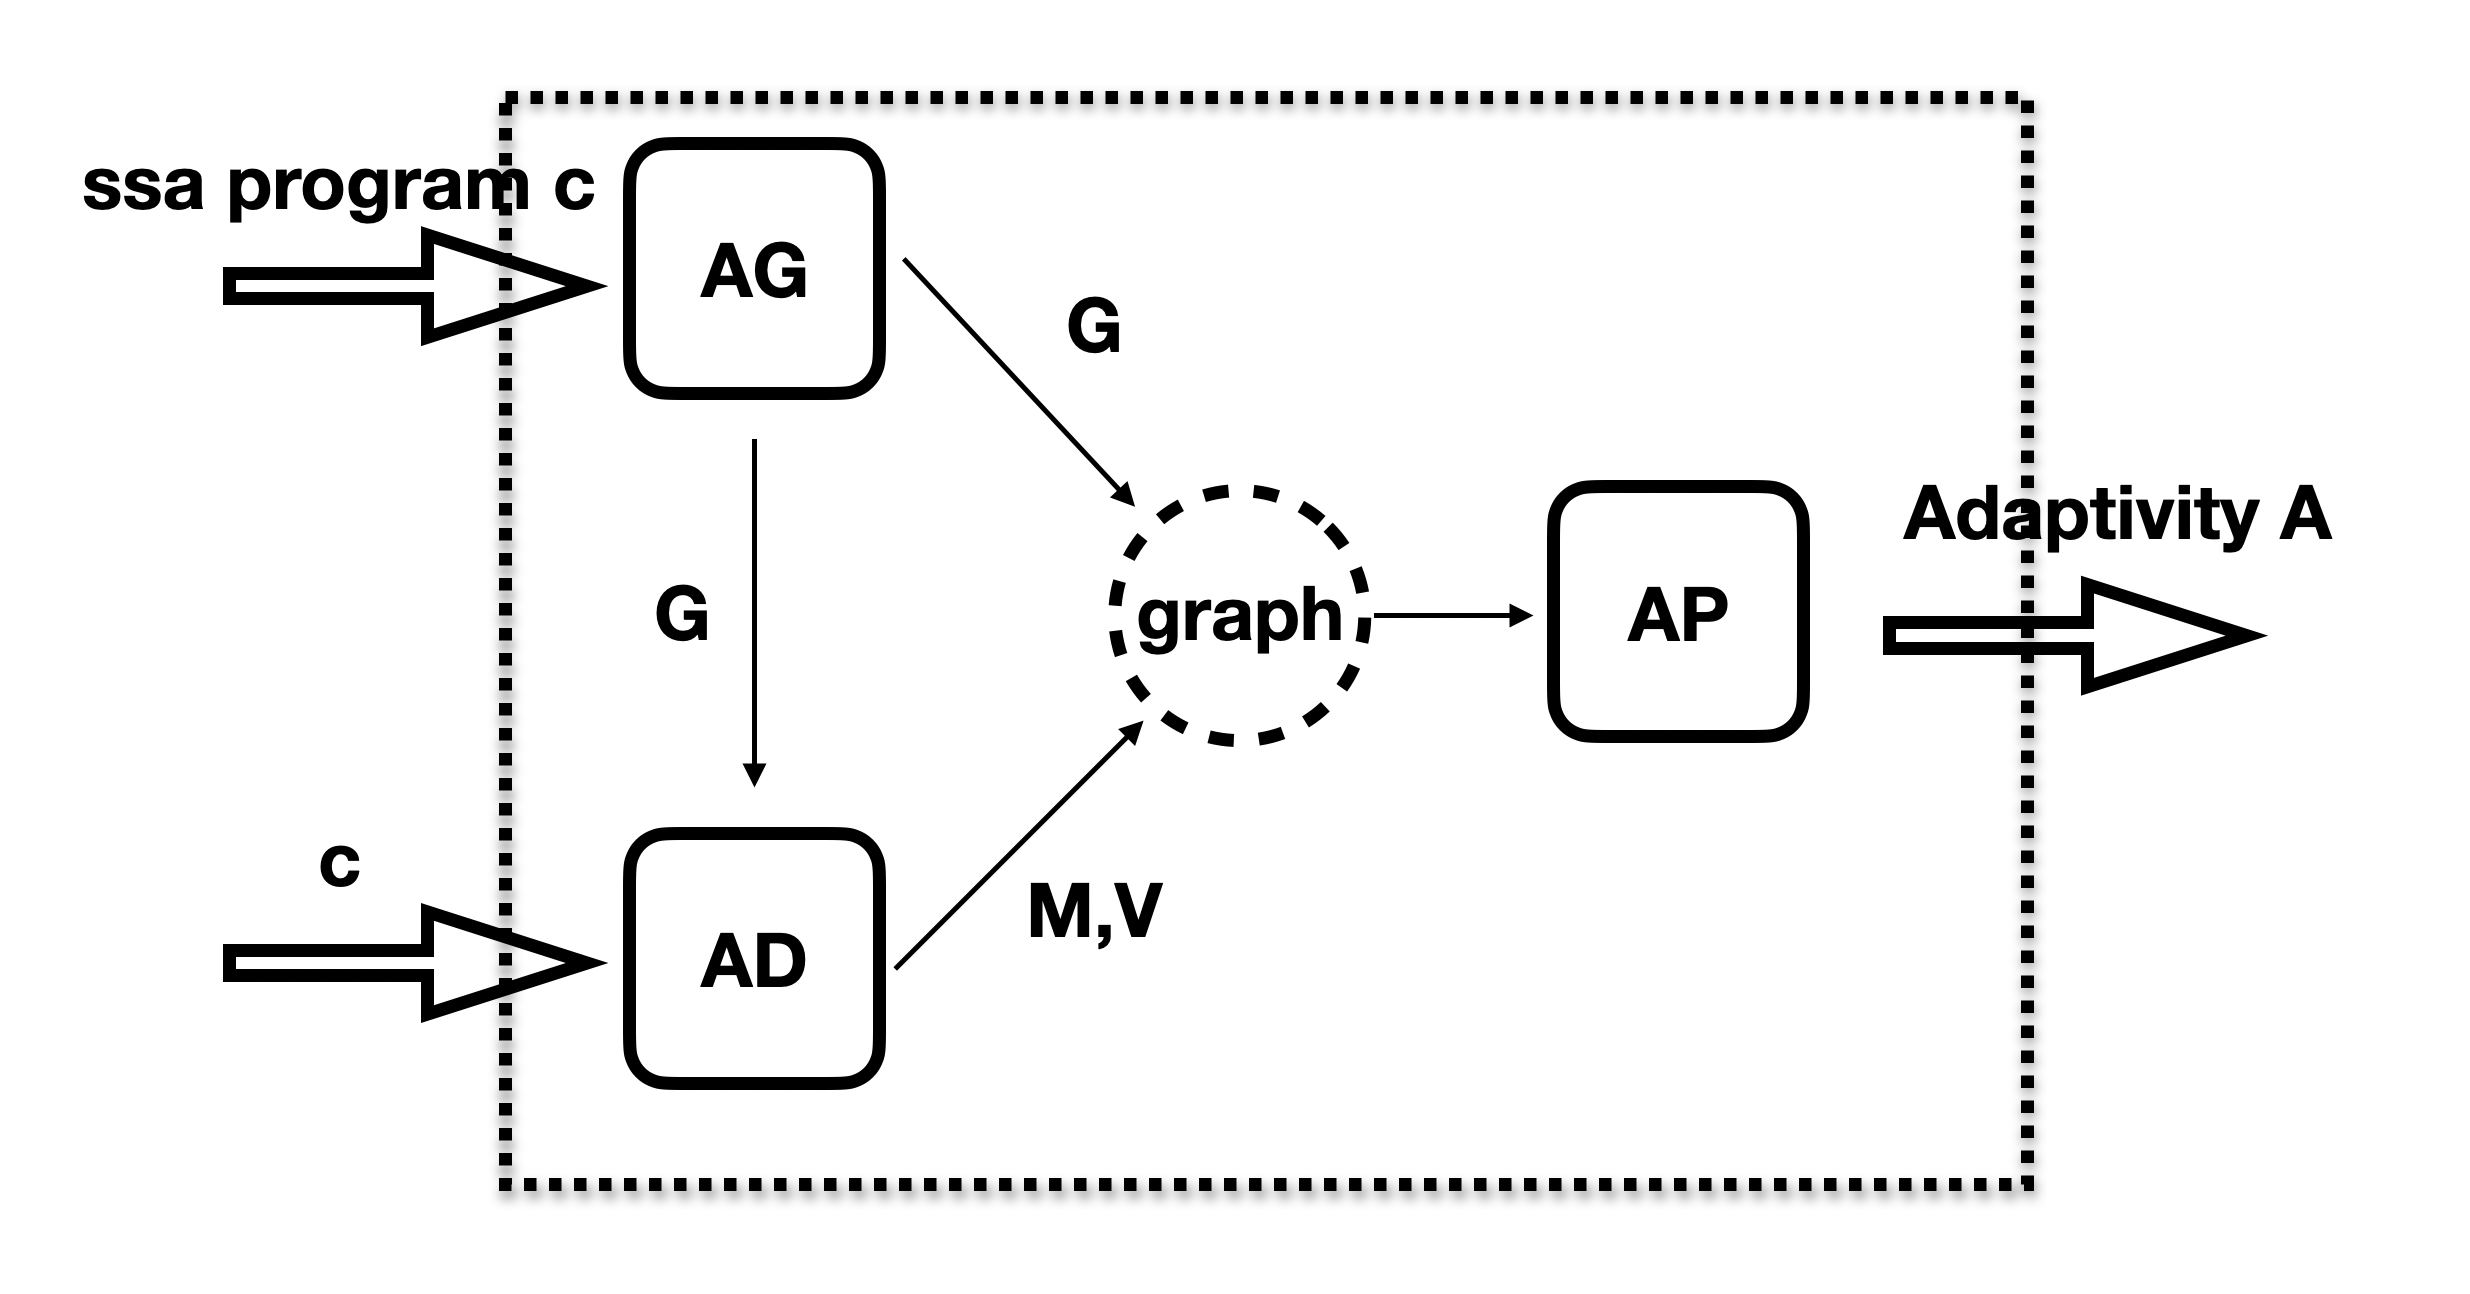
\includegraphics[width=1.0\columnwidth]{adapfun.png}
  \vspace{-0.3cm}
  \caption{The overview of {\THESYSTEM}}
  \label{fig:adaptfun}
  \vspace{-0.5cm}
\end{figure}

\begin{enumerate}
  % \item The data dependency relation analysis through the static data flow analysis technique.
  % \item The dependency quantity analysis through the static program reachability bound analysis techniques.
  % \item The program adaptivity estimation, through newly designed algorithms based on the results estimated above, 
  % computing the adaptivity upper bound soundly 
  % and accurately.
  \item \textbf{\emph{Dependency Relation} Estimation} in Section~\ref{sec:static-dep}.
  In order to accurately estimate the adaptivity,  {\THESYSTEM} first estimates
  %  the \emph{dependency relation} 
  %  Corresponding to the {\THESYSTEM} analyzes 
  the data \emph{dependency relation} through the static data flow analysis technique in Section~\ref{sec:static-dep}.
  This analysis step corresponds to the first step in execution-based adaptivity analysis. 
  The estimated result produced from 
  this step is proved as a sound upper bound for the variable \emph{may-dependency} relation in Definition~\ref{def:var_dep} from execution-based analysis in Section~\ref{sec:dynamic-datadep}.
  \item \textbf{\emph{Dependency Quantity} Estimation} in Section~\ref{sec:static-quantity}.
  % Still , 
  Corresponding to the second step in execution-based adaptivity analysis, {\THESYSTEM} then estimates the \emph{dependency quantity} 
  % is estimated by {\THESYSTEM} 
  through the static program reachability bound analysis techniques.
  %
  For every labeled variable and every pair of labeled variables with estimated dependency relation, this analysis provides the symbolic
 bounds on their reaching times during the program execution.
  % , in Section~\ref{sec:static-quantity}.
  % This analysis corresponds to the second step in execution-based adaptivity analysis. 
  The estimated result produced from 
  this step is proved as a sound upper bound for the reachability-bound from execution-based analysis as well.
  \item \textbf{\emph{Adaptivity} Estimation} in Section~\ref{sec:static-adapt}.
  % The program  estimation, 
  % In 
  The static program adaptivity analysis in this step
  % , specifically estimating 
  estimates the \emph{adaptivity} formalized in Definition~\ref{def:trace_adapt}, in following two steps:
  \begin{itemize}
  %  is presented in Section~\ref{sec:static-reachability}.
  % the program adaptivity estimation, 
  \item According to the third step of execution-based adaptivity analysis, 
  {\THESYSTEM} in this step first builds a similar graph to {over-}approximate the
  % execution-based dependency graph (in Definition~\ref{def:trace_graph})
  Execution-Based Dependency Graph (in Definition~\ref{def:trace_graph})
  \\
  This graph is built over the same vertices set as the execution-based dependency graph, which is program's set of labeled variables with unique labels.
  \\
  Then it builds the edges between vertices 
  % consider both control flow and data flow, generated in
  using the estimated dependency relation from Section~\ref{sec:static-dep}.
  % which is the same set as the vertices in the execution-based dependency graph extracted directly from the program
  %  constructs a program-based dependence graph for approximating the execution-based dependency graph.
  %  in Section~\ref{sec:dynamic-adapt}.
  \\
  Then according to the estimated reachability bound for every labeled variable and every pair of labeled variables with estimated dependency relation
  from Section~\ref{sec:static-quantity}, it assigns weight for every vertex and every edge on this graph.
  \\
  Overall, this program-based graph has a similar topology structure as 
  % the one
  % of 
  the Execution-Based Dependency Graph. It has the same
  vertices and query annotations, but approximated edges and weights. We call the graph generated by static analysis techniques, static analysis dependency graph. 
\item Then, based on this graph, {\THESYSTEM} 
    computes the adaptivity upper bound soundly 
    and accurately through a newly designed algorithm.
\\
Likewise, the adaptivity is defined as a finite walk in the execution based dependency graph, 
our static estimation on this adaptivity also relies on finding a path in the static analysis dependency graph.
The construction of the static analysis dependency graph is of great value of showing some useful properties of the target program,
such as dependency between variables, 
the execution upper bound of a certain command, while the key novelty is our path searching algorithm,
which connects all the information we need in the static analysis dependency graph and provides us a sound over-estimation of adaptivity! 
In order to get a sound but precise upper bound, 
we will discuss some challenges in finding the 'appropriate' path in the graph, 
and how our algorithm responds to these challenges.
I present the path searching algorithm in Section~\ref{sec:static-adapt}.
  \end{itemize}
  \end{enumerate}
% \subsubsection{Graph Estimation}
%
%
% According to the dependency graph we use in adaptivity definition, we want to build a similar graph to {over-}approximate the
% % execution-based dependency graph (in Definition~\ref{def:trace_graph})
% Execution-Based Dependency Graph (in Definition~\ref{def:trace_graph}). The construction considers the vertices, edges, and the weight of every node, as well as some annotations which marks the query usage. The overall picture of this step is organized as follows.
% % through Section~\ref{sec:alg_vertexgen}, Section~\ref{sec:alg_weightedgegen} and~\ref{sec:alg_graphgen}:


% \begin{enumerate}
% \item  Vertices are the program's labeled variables with unique labels,
% which is the same set as the vertices in the execution-based dependency graph extracted directly from the program
% % , see Section~\ref{sec:static-adapt}
% % without extra static analysis technique.
% % \item Query annotations are also decided directly from the program, when there is a query request, the associated variables which are the results of the query requests are marked in the form of a flag, $0$ means no query, $1$ represents query related. See Section~\ref{sec:alg_vertexgen}.
% \item The edges between vertices consider both control flow and data flow, generated in
% Section~\ref{sec:static-dep}
% \item Every 
% vertex has a weight, which tells the maximal times that this vertex can be reached in realistic execution.
% This weight is estimated by a reachability bound analysis on each vertex, See Section~\ref{sec:static-quantity}.
% \item Every 
% vertex has a weight, which tells the maximal times that this vertex can be reached in realistic execution.
% This weight is estimated by a reachability bound analysis on each vertex, See Section~\ref{sec:static-quantity}.

% \item  Finally, with all the ingredients ready, we construct the final approximated program-based dependency graph in Section~\ref{sec:static-adapt}
% \end{enumerate}

% % the algorithm  without extra static analysis technique.
% % \\
% Overall, this program-based graph has a similar topology structure as 
% % the one
% % of 
% the Execution-Based Dependency Graph. It has the same
% vertices and query annotations, but approximated edges and weights. We call the graph generated by static analysis techniques, static analysis dependency graph. 

% \subsubsection{Adaptivity Computation}

% Likewise the adaptivity is defined as a finite walk in the execution based dependency graph, 
% our static estimation on this adaptivity also relies on finding a path in the static analysis dependency graph.
% The construction of the stastic analysis dependency graph is of great value of showing some useful properties of the target program, such as dependency between variables, 
% the execution upper bound of a certian command, while the key novelty is our path searching algorithm, which connects all the information we need in the static analysis dependency graph and provides us a sound over-estimation of adaptivity! 
% In order to get a sound but precise upper bound, 
% we will discuss some challenges in finding the 'appropriate' path in the graph, and how our algorithm responds to these challenge. We present the path searching algorithm in Section~\ref{sec:static-adapt}.